\chapter{ARDC in practice}
\label{ch:ardc}

We now have everything we need to do the work: an archive that keeps source code for the long
term, and an intrinsic identifier that names exactly the code we mean. This chapter is the
operational heart of the note. It turns the principle ``treat software as a first-class output''
into four concrete verbs you can apply to a repository of your choice --- your own code, a library
you depend on, a result you want to cite. The verbs are \textbf{A}rchive, \textbf{R}eference,
\textbf{D}escribe, and \textbf{C}ite~\&~credit; together they spell \textsc{ardc}, and each ends
with a hands-on lab.

\takeaway{Archive once; then reference at the granularity your claim needs.}

\section{Archive}

Recall the one hard requirement from the CODE roadmap: \emph{publish and archive}. Publishing on a
forge you already do. Archiving means depositing the code, with its history, into Software
Heritage, and there are four ways in, in rising order of automation~\autocite{SwhCACM2018}.

The simplest is \emph{Save Code Now}: go to \url{https://save.softwareheritage.org}, paste the
clone URL of a public repository, and the archive will visit it --- Git, Mercurial, Subversion, no
matter. One step better is the \emph{updateswh} browser extension, which puts a single ``archive
this'' button on the repository pages of GitHub, GitLab, and Bitbucket. Better still, for code you
maintain, is a \emph{webhook}: wire your forge so that every release triggers archival
automatically, and you never have to remember again. And there is a fourth channel, the
\textsc{sword}-based \emph{deposit} (\url{https://deposit.softwareheritage.org}) --- but it is
\emph{not} a general path: it is reserved for trusted partners and registered organizations ---
a journal, an institution, HAL --- who hold credentials to push a tarball with its metadata
straight into the archive. An ordinary researcher does not have those credentials, and does not
need them: the easy paths below cover exactly the case the deposit was built to handle.

\subsection*{When all you have is a tarball}

The three public channels above all assume one thing: that your code lives in a forge, behind a
clone URL. \emph{And yet} a great deal of research software does not --- it is a \texttt{.zip} or
\texttt{.tar.gz} attached to a paper, a snapshot with no public Git remote. For that case, two
paths are open to you, and neither needs partner credentials.

The easiest, by far, is to go through \emph{Zenodo}. Since the Zenodo--Software Heritage
integration launched in late 2024, software you deposit on Zenodo is \emph{automatically} sent on
to Software Heritage, provided the files are publicly accessible; Software Heritage computes its
\textsc{swhid}, and Zenodo links that \textsc{swhid} to the record's \textsc{doi} and shows both on
the landing page~\autocite{zenodoswh2024}. So you upload your archive once, and walk away with
\emph{both} identifiers --- the \textsc{doi} for discoverability in the scholarly literature, and
the \textsc{swhid} for the verifiable identity of the exact bytes. It is the same division of
labour we have insisted on throughout: \emph{a \textsc{doi} for findability, a \textsc{swhid} for
integrity} --- and here you get both, for the price of one upload, with no forge required.

The second path stays inside Software Heritage: \emph{Save Code Now} can also ingest a
\texttt{.zip} or tarball directly, rather than a clone URL --- but this is gated. It is open to
registered accounts holding the \emph{ambassador} role, which Software Heritage grants on request
(the account is free); an anonymous visitor can submit only a version-control
URL.\footnote{See the \textsc{faq}: \url{https://docs.softwareheritage.org/user/faq/index.html}.}
If you expect to archive tarballs regularly --- shepherding a journal's artifacts, say --- this
is worth setting up; for a one-off, the Zenodo route is simpler. Either way, the full recipe lives
in the online
HOWTO.\footnote{\url{https://www.softwareheritage.org/how-to-archive-reference-code/}}

However the code got in, the result is the same: it is now kept, and it now has a name.

\begin{handson}[Hands-on: archive any repository, and automate it]
\begin{enumerate}[nosep,leftmargin=*]
  \item Pick a repository worth keeping --- your own, or one you depend on. Archive it with the
        \textbf{updateswh} extension or at \url{https://save.softwareheritage.org}; wait for the
        visit to reach status \texttt{full}.
  \item Then make it automatic: add a release \emph{webhook} (GitHub, GitLab, Gitea, Bitbucket,
        SourceForge) so each new tag is archived without your lifting a finger.
\end{enumerate}
\end{handson}

\section{Reference}

Archiving gives the code a name; \emph{referencing} is the craft of choosing \emph{which} name to
quote, and at what granularity. Here the identifiers of Chapter~\ref{ch:identifiers} come into
their own, because a paper rarely depends on ``the repository'' --- it depends on something far
more specific. Match the identifier to the claim~\autocite{cise-2020-doi}:

\begin{description}[leftmargin=!,labelwidth=2.6cm,font=\bfseries\sffamily]
  \item[the project] ``Inria created OCaml and Scikit-learn'' --- name the project (a \texttt{snp},
        or the origin).
  \item[a release] ``2D Voronoi diagrams were introduced in CGAL 3.1.0'' --- name the release
        (\texttt{rel}).
  \item[an exact state] ``this result was produced using commit 0064fbd\ldots'' --- name the
        revision (\texttt{rev}).
  \item[a code fragment] ``the core algorithm is in lines 101--143 of \texttt{parmap.ml} in commit
        0064fbd\ldots'' --- name the content, with \texttt{path} and \texttt{lines}.
\end{description}

For a paper you will usually want a \emph{qualified} \textsc{swhid}: the core name that identifies,
plus the \texttt{origin}, \texttt{visit}, and \texttt{anchor} qualifiers that let a reader walk
straight to it in the archive and see where it came from. And when no precise version is known ---
when you simply want to point at ``the project, as the archive saw it'' --- an origin-qualified
\textsc{swhid} serves as a Wayback-machine-style pointer into the crawl history.

\begin{handson}[Hands-on: reference code in a paper]
Take a result of your own that rests on code, and build its reference with the Rust reference tool
\texttt{swhid-rs} (\texttt{cargo install swhid}; see Appendix~\ref{app:swhid-tools}). Compute the
\texttt{cnt} \textsc{swhid} of the precise file --- \texttt{swhid content -{}-file analysis.py} ---
and the \texttt{rev} \textsc{swhid} of the exact commit, which is simply \swhid{swh:1:rev:}
prepended to \texttt{git rev-parse HEAD}. Add the \texttt{path} and \texttt{lines} qualifiers by
hand, then paste each qualified \textsc{swhid} into \texttt{https://archive.softwareheritage.org/}
and confirm it highlights exactly the code you meant.
\end{handson}

\section{Describe}

A name keeps code findable; \emph{description} makes it understandable and reusable, and it is
where a little effort pays off enormously. Three files do most of the work, and you should add them
in order of growing ambition~\autocite{boettiger2017codemeta}.

Start with a \texttt{README}: the human entry point, answering \emph{what, why, install, run, cite,
licence} in plain words --- ten minutes today, and the single highest-value thing you can do. As a
project grows, add a \texttt{codemeta.json}: a rich, machine-readable description --- authors,
dependencies, funding, archival identifiers --- in a schema.org-based vocabulary that forges and
Software Heritage can read to generate citations automatically. Do not write it by hand; use the
CodeMeta Generator.\footnote{\url{https://codemeta.github.io/codemeta-generator/}} From the
CodeMeta file you can in turn generate a \texttt{CITATION.cff}, the lightweight format that makes
GitHub show a ``Cite this repository'' button~\autocite{druskat2021cff}.

And do not forget the licence --- the most consequential one-line file in your repository. By the
Berne Convention, code is copyrighted the moment it is written, and the default is \emph{all rights
reserved}: without a licence, nobody may legally reuse your work, however open you meant it to be.
Yet roughly \emph{ninety per cent of public repositories on GitHub carry no licence at all}. Choose
one --- permissive (MIT, BSD, Apache-2.0) or copyleft (the GPL family) --- declare it
machine-readably with an \textsc{spdx} identifier, and, if you like, automate the bookkeeping with
the REUSE specification. (Resist the temptation to reach for Creative Commons: it was not designed
for software.) The community has distilled all of this into the FAIR Software Five
recommendations.\footnote{\url{https://fair-software.eu/}}

\takeaway{About 90\% of public repositories carry no licence --- so by default nobody may legally
reuse them. A one-line \textsc{spdx} tag fixes it.}

To put your software forward as a citable output --- onto your CV, into your institution's portal
and the literature --- one further step helps: reference it in a curated catalogue. In France that
means depositing in HAL, which is wired directly into Software Heritage
(Figure~\ref{fig:hal-swh}); elsewhere, registries such as OSPO-RADAR play the same role.

\begin{figure}[htbp]
  \centering
  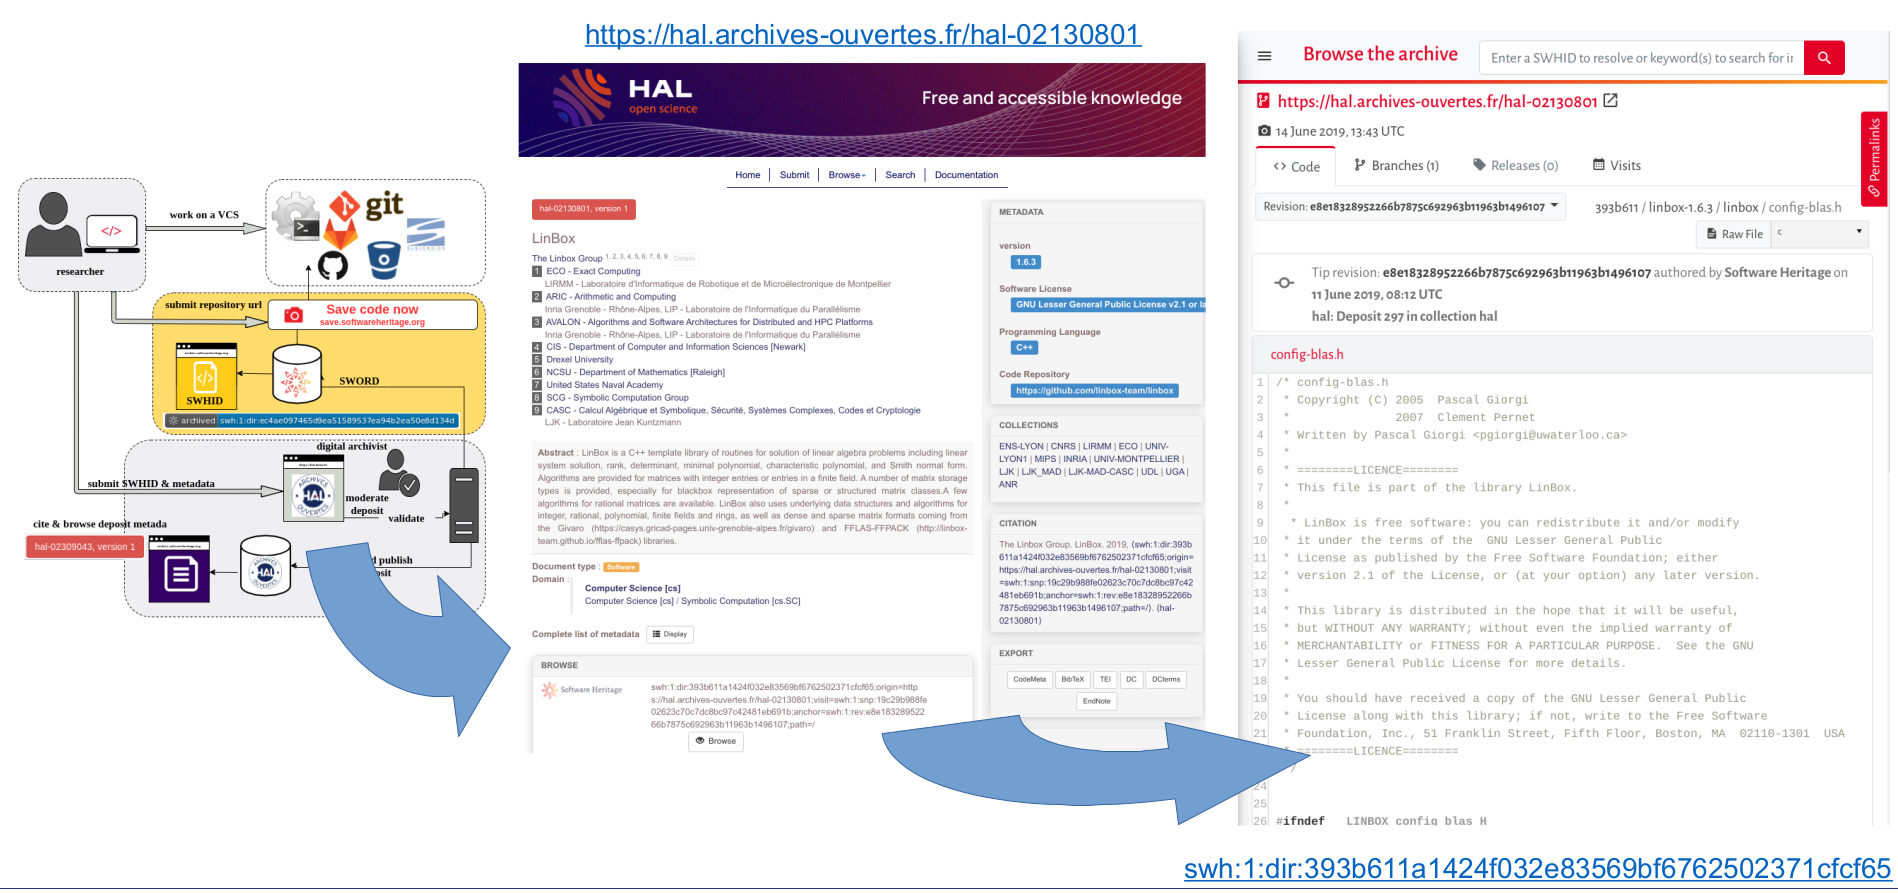
\includegraphics[width=.92\linewidth]{figures/hal-swh-overview.png}
  \caption[HAL and Software Heritage]{The HAL\,/\,Software Heritage synergy: a researcher deposits a
  curated record of a piece of software in the HAL open-access portal, while the source code itself
  is archived in Software Heritage --- the two linked by the code's \textsc{swhid}.}
  \label{fig:hal-swh}
\end{figure}

\begin{handson}[Hands-on: describe, and watch the citation appear]
Create a \texttt{codemeta.json} with the CodeMeta Generator, commit it, and re-archive the
repository. Then open the project in the Software Heritage archive and watch the citation panel
populate from your metadata --- and use it to produce the citation you actually want.
\end{handson}

\section{Cite and credit}

Finally, cite software as you would cite anything else in research: in the bibliography, as a
first-class reference. For decades there was no proper way to do this, and software citations were
forced into \texttt{@misc} entries that lost the version, the licence, and any verifiable
identifier~\autocite{2020GtCitation}. The \texttt{biblatex-software} style fixes
that~\autocite{DiCosmoSEN2020}. It adds four entry types --- \texttt{@software} for a project,
\texttt{@softwareversion} for a release, \texttt{@softwaremodule} for a component, and
\texttt{@codefragment} for a precise span of code --- chained with \texttt{crossref} so shared
metadata is written once, and, decisively, it carries a \texttt{swhid=} field. The package is on
CTAN and in TeX\,Live, and has shipped in the ACM \texttt{acmart} class since 2022, so the
\textsc{swhid} renders natively in an ACM paper (Figure~\ref{fig:biblatex-swh}).

\begin{figure}[htbp]
  \centering
  
\includegraphics[width=.9\linewidth]{figures/BibLaTeX-swh.png}
  \caption[Software in a bibliography, done right]{A software bibliography typeset with
  \texttt{biblatex-software}: each entry carries its version, licence, repository, and ---
  decisively --- a \textsc{swhid}, so the citation still resolves to the exact code long after the
  project's URL has rotted.}
  \label{fig:biblatex-swh}
\end{figure}

The payoff is that a software citation becomes \emph{reproducible}: a \textsc{swhid} in the
bibliography resolves to the exact bytes you used, with no dependence on a URL that may not outlive
the paper. This note's own bibliography is built this way --- the Parmap library, for instance, is
cited as a versioned software entry carrying its \textsc{swhid}, and a routine within it as a code
fragment.\footnote{See the \texttt{biblatex-software} entries~\autocite{parmap-1.1.1,simplemapper}
in the references.}

\takeaway{A \textsc{swhid} in the bibliography is a citation that still resolves when the URL is
gone.}

\begin{handson}[Hands-on: cite software with biblatex-software]
\begin{enumerate}[nosep,leftmargin=*]
  \item Write a \texttt{@softwareversion} entry for the code you archived, with its \texttt{swhid=}
        field; add a \texttt{@codefragment} child via \texttt{crossref} for a specific routine.
  \item Produce the variants --- a project-level \texttt{@software}, a \texttt{@softwaremodule} ---
        and compare how each renders.
  \item Drop the entries into an \texttt{acmart} article and confirm the \textsc{swhid} renders in
        the ACM template.
\end{enumerate}
\end{handson}

That is \textsc{ardc}: archive the code, reference it precisely, describe it, and cite it --- a
practice you can adopt incrementally, starting, as we keep saying because it is true, with your next
paper. The remaining question is what all this rigour \emph{buys} us. The answer, and the sharpest
test of the whole approach, is reproducibility and the evaluation of research artifacts: the
subject of the next chapter.
